% Options for packages loaded elsewhere
\PassOptionsToPackage{unicode}{hyperref}
\PassOptionsToPackage{hyphens}{url}
%
\documentclass[
]{book}
\usepackage{amsmath,amssymb}
\usepackage{iftex}
\ifPDFTeX
  \usepackage[T1]{fontenc}
  \usepackage[utf8]{inputenc}
  \usepackage{textcomp} % provide euro and other symbols
\else % if luatex or xetex
  \usepackage{unicode-math} % this also loads fontspec
  \defaultfontfeatures{Scale=MatchLowercase}
  \defaultfontfeatures[\rmfamily]{Ligatures=TeX,Scale=1}
\fi
\usepackage{lmodern}
\ifPDFTeX\else
  % xetex/luatex font selection
\fi
% Use upquote if available, for straight quotes in verbatim environments
\IfFileExists{upquote.sty}{\usepackage{upquote}}{}
\IfFileExists{microtype.sty}{% use microtype if available
  \usepackage[]{microtype}
  \UseMicrotypeSet[protrusion]{basicmath} % disable protrusion for tt fonts
}{}
\makeatletter
\@ifundefined{KOMAClassName}{% if non-KOMA class
  \IfFileExists{parskip.sty}{%
    \usepackage{parskip}
  }{% else
    \setlength{\parindent}{0pt}
    \setlength{\parskip}{6pt plus 2pt minus 1pt}}
}{% if KOMA class
  \KOMAoptions{parskip=half}}
\makeatother
\usepackage{xcolor}
\usepackage{color}
\usepackage{fancyvrb}
\newcommand{\VerbBar}{|}
\newcommand{\VERB}{\Verb[commandchars=\\\{\}]}
\DefineVerbatimEnvironment{Highlighting}{Verbatim}{commandchars=\\\{\}}
% Add ',fontsize=\small' for more characters per line
\usepackage{framed}
\definecolor{shadecolor}{RGB}{248,248,248}
\newenvironment{Shaded}{\begin{snugshade}}{\end{snugshade}}
\newcommand{\AlertTok}[1]{\textcolor[rgb]{0.94,0.16,0.16}{#1}}
\newcommand{\AnnotationTok}[1]{\textcolor[rgb]{0.56,0.35,0.01}{\textbf{\textit{#1}}}}
\newcommand{\AttributeTok}[1]{\textcolor[rgb]{0.13,0.29,0.53}{#1}}
\newcommand{\BaseNTok}[1]{\textcolor[rgb]{0.00,0.00,0.81}{#1}}
\newcommand{\BuiltInTok}[1]{#1}
\newcommand{\CharTok}[1]{\textcolor[rgb]{0.31,0.60,0.02}{#1}}
\newcommand{\CommentTok}[1]{\textcolor[rgb]{0.56,0.35,0.01}{\textit{#1}}}
\newcommand{\CommentVarTok}[1]{\textcolor[rgb]{0.56,0.35,0.01}{\textbf{\textit{#1}}}}
\newcommand{\ConstantTok}[1]{\textcolor[rgb]{0.56,0.35,0.01}{#1}}
\newcommand{\ControlFlowTok}[1]{\textcolor[rgb]{0.13,0.29,0.53}{\textbf{#1}}}
\newcommand{\DataTypeTok}[1]{\textcolor[rgb]{0.13,0.29,0.53}{#1}}
\newcommand{\DecValTok}[1]{\textcolor[rgb]{0.00,0.00,0.81}{#1}}
\newcommand{\DocumentationTok}[1]{\textcolor[rgb]{0.56,0.35,0.01}{\textbf{\textit{#1}}}}
\newcommand{\ErrorTok}[1]{\textcolor[rgb]{0.64,0.00,0.00}{\textbf{#1}}}
\newcommand{\ExtensionTok}[1]{#1}
\newcommand{\FloatTok}[1]{\textcolor[rgb]{0.00,0.00,0.81}{#1}}
\newcommand{\FunctionTok}[1]{\textcolor[rgb]{0.13,0.29,0.53}{\textbf{#1}}}
\newcommand{\ImportTok}[1]{#1}
\newcommand{\InformationTok}[1]{\textcolor[rgb]{0.56,0.35,0.01}{\textbf{\textit{#1}}}}
\newcommand{\KeywordTok}[1]{\textcolor[rgb]{0.13,0.29,0.53}{\textbf{#1}}}
\newcommand{\NormalTok}[1]{#1}
\newcommand{\OperatorTok}[1]{\textcolor[rgb]{0.81,0.36,0.00}{\textbf{#1}}}
\newcommand{\OtherTok}[1]{\textcolor[rgb]{0.56,0.35,0.01}{#1}}
\newcommand{\PreprocessorTok}[1]{\textcolor[rgb]{0.56,0.35,0.01}{\textit{#1}}}
\newcommand{\RegionMarkerTok}[1]{#1}
\newcommand{\SpecialCharTok}[1]{\textcolor[rgb]{0.81,0.36,0.00}{\textbf{#1}}}
\newcommand{\SpecialStringTok}[1]{\textcolor[rgb]{0.31,0.60,0.02}{#1}}
\newcommand{\StringTok}[1]{\textcolor[rgb]{0.31,0.60,0.02}{#1}}
\newcommand{\VariableTok}[1]{\textcolor[rgb]{0.00,0.00,0.00}{#1}}
\newcommand{\VerbatimStringTok}[1]{\textcolor[rgb]{0.31,0.60,0.02}{#1}}
\newcommand{\WarningTok}[1]{\textcolor[rgb]{0.56,0.35,0.01}{\textbf{\textit{#1}}}}
\usepackage{longtable,booktabs,array}
\usepackage{calc} % for calculating minipage widths
% Correct order of tables after \paragraph or \subparagraph
\usepackage{etoolbox}
\makeatletter
\patchcmd\longtable{\par}{\if@noskipsec\mbox{}\fi\par}{}{}
\makeatother
% Allow footnotes in longtable head/foot
\IfFileExists{footnotehyper.sty}{\usepackage{footnotehyper}}{\usepackage{footnote}}
\makesavenoteenv{longtable}
\usepackage{graphicx}
\makeatletter
\def\maxwidth{\ifdim\Gin@nat@width>\linewidth\linewidth\else\Gin@nat@width\fi}
\def\maxheight{\ifdim\Gin@nat@height>\textheight\textheight\else\Gin@nat@height\fi}
\makeatother
% Scale images if necessary, so that they will not overflow the page
% margins by default, and it is still possible to overwrite the defaults
% using explicit options in \includegraphics[width, height, ...]{}
\setkeys{Gin}{width=\maxwidth,height=\maxheight,keepaspectratio}
% Set default figure placement to htbp
\makeatletter
\def\fps@figure{htbp}
\makeatother
\setlength{\emergencystretch}{3em} % prevent overfull lines
\providecommand{\tightlist}{%
  \setlength{\itemsep}{0pt}\setlength{\parskip}{0pt}}
\setcounter{secnumdepth}{5}
\providecommand{\arrowvert}{}
\usepackage{booktabs}
\usepackage{fancyhdr}
\usepackage{geometry}
\usepackage{titlesec}
\usepackage{etoolbox}
\usepackage{mathptmx}
\geometry{
  top=1in, 
  bottom=1in, 
  left=1in, 
  right=1in, 
  headheight=17pt, 
  includehead, 
  includefoot  
}
\pagestyle{fancy}
\fancyhf{} 
\fancyhead[R]{\thepage} 
\renewcommand{\headrulewidth}{0pt} 
\fancypagestyle{plain}{
  \fancyhf{}
  \fancyhead[R]{\thepage}
  \renewcommand{\headrulewidth}{0pt}
}

\makeatletter
\patchcmd{\chapter}{\if@openright\cleardoublepage\else\clearpage\fi}{\clearpage}{}{}
\makeatother


\titleformat{\section}
  {\normalfont\Large\bfseries\itshape}{\thesection}{1em}{}
\titleformat{\subsection}
  {\normalfont\large\itshape\bfseries}{\thesubsection}{1em}{}
  
\ifLuaTeX
  \usepackage{selnolig}  % disable illegal ligatures
\fi
\usepackage[]{natbib}
\bibliographystyle{plainnat}
\IfFileExists{bookmark.sty}{\usepackage{bookmark}}{\usepackage{hyperref}}
\IfFileExists{xurl.sty}{\usepackage{xurl}}{} % add URL line breaks if available
\urlstyle{same}
\hypersetup{
  pdftitle={A Scientific Way to Build a Likable Studying Music Playlist},
  pdfauthor={Junqi Fu},
  hidelinks,
  pdfcreator={LaTeX via pandoc}}

\title{A Scientific Way to Build a Likable Studying Music Playlist}
\author{Junqi Fu}
\date{2023-12-10}

\begin{document}
\maketitle

{
\setcounter{tocdepth}{1}
\tableofcontents
}
\hypertarget{background}{%
\chapter{Background}\label{background}}

In 2021, Spotify disclosed in an official survey report that approximately 87\% of participants in the U.S. and U.K. indicated that audio plays a significant role in enhancing productivity during various tasks, such as studying \citep{Spotify2021}. Between 2020 and 2021, Spotify noted a 26\% rise in user-generated ``focus'' playlists on its platform worldwide. This increase underscores the growing functional role of music in the lives of users \citep{Spotify2021}.

\begin{figure}
\centering
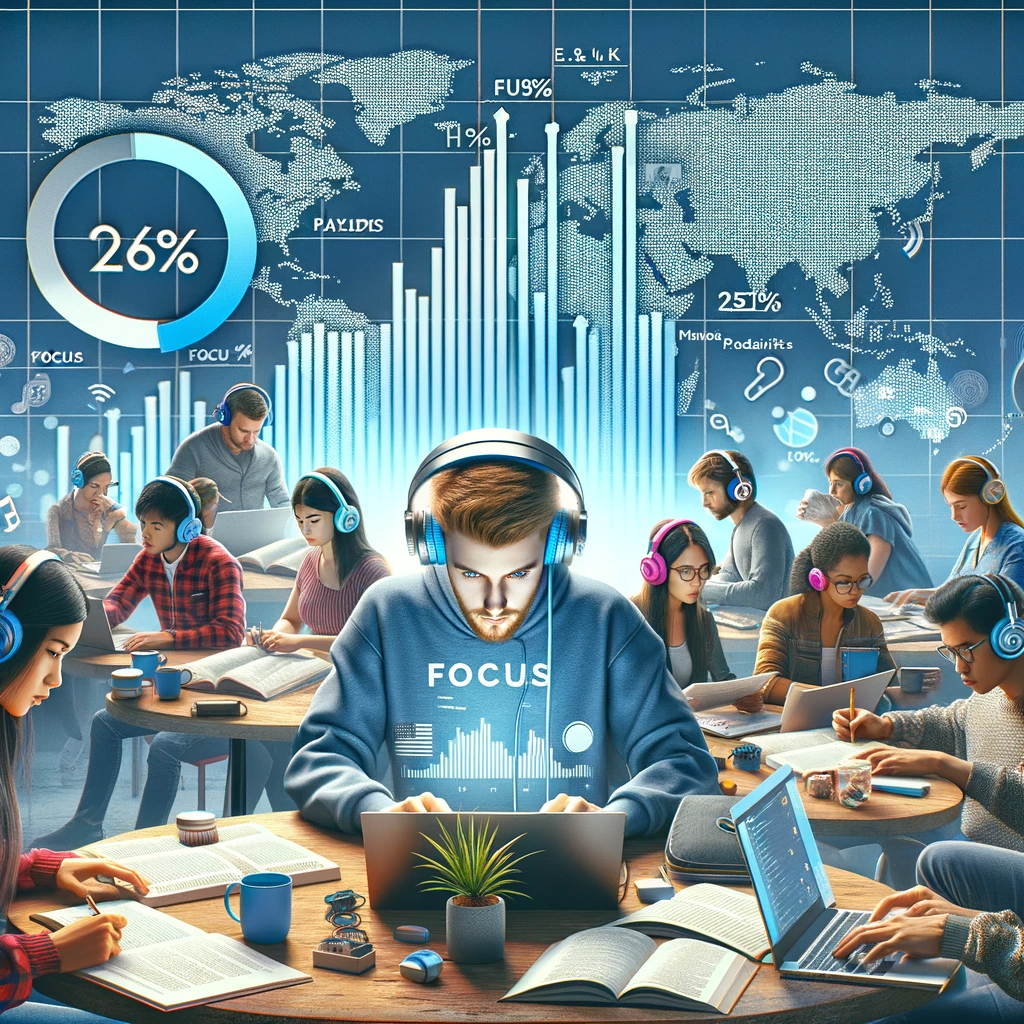
\includegraphics{1.png}
\caption{Significant role of audio in enhancing productivity. Generated by DALL.E 3}
\end{figure}

\hypertarget{music-cognitive-perofrmance}{%
\section{Music \& Cognitive Perofrmance}\label{music-cognitive-perofrmance}}

Although there are differing opinions regarding the moderate effects of specific musical features and genres on enhancing cognitive tasks, cognitive scientists have found evidence that background music helps to increase workers' concentration and cognitive performance during work \citep[e.g.,][]{Huang2011EffectsOB, NationalUniversity2021}. According to \citet{NationalUniversity2021}, background music can activate both the left and right sides of the brain simultaneously, leading to maximized learning and improved memory. Additionally, music often indirectly influences cognitive performance through its significant impact on users' mood, blood pressure, and other physiological responses.

\hypertarget{music-eudaimonia}{%
\section{Music \& Eudaimonia}\label{music-eudaimonia}}

Additionally, empirical research has explored the significant relationship between music and the experience of complicated emotional responses in users, such as self-transcendent emotions or eudaimonia.

Self-transcendent emotions are a category of human emotions, including feelings like admiration, gratitude, hope, and inspiration. These emotions lead individuals to focus less on themselves and more on the needs of others \citep[e.g.,][]{felnhofer2013game, stellar2017self, vancappellen2013positive}. Unlike other positive emotions, they possess a eudaimonic nature. By inducing a departure from our habitual cognitive patterns, self-transcendent emotions are capable of catalyzing our motivation towards both personal growth and the advancement of humanity's collective well-being \citep{algoe2009witnessing}.

Cognitive scientists has found that significant relationship between long-term music engagement and development of self-transcendent/eudaimonia emotions. For example,
\citet{nijs2021flourishing} explores how musical activities combined with movement practices (e.g., gospel music) can help young adults develop eudaimonic values such as self-awareness and a strong sense of belonging and bonding within their community. Furthermore, \citet{verneert2021space}'s two-year study found that a sense of empathy, collective belonging, and meaningfulness develops in individuals when they continuously participate in collective improvisation with homeless adults and individuals facing emotional, psychological, and cognitive challenges.

\begin{figure}
\centering
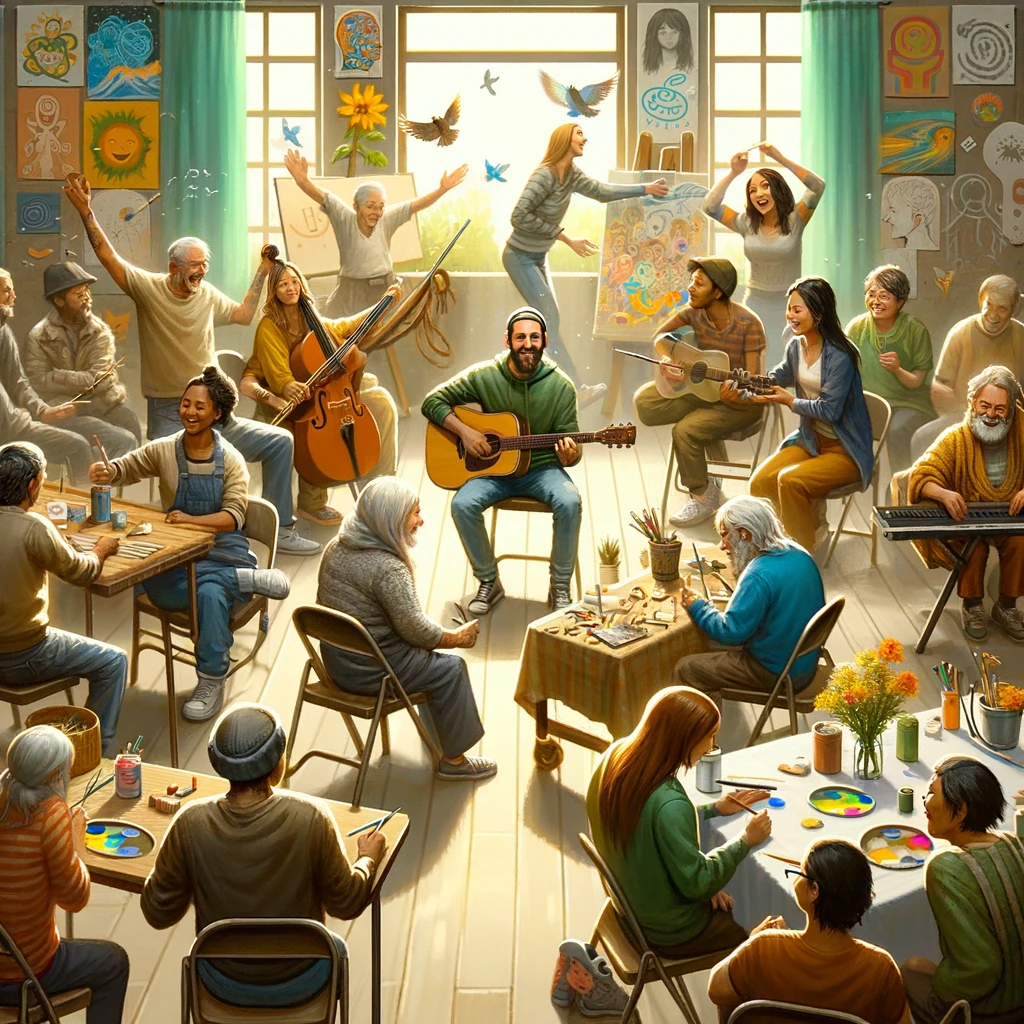
\includegraphics{2.png}
\caption{Collective improvisation enhances a sense of empathy, collective belonging, and meaningfulness. Generated by DALL.E 3}
\end{figure}

\hypertarget{a-scientific-way-to-build-a-likable-studying-music-playlist-for-an-upcoming-cognitive-flow-study}{%
\section{A Scientific Way to Build a Likable Studying Music Playlist For An Upcoming Cognitive Flow Study}\label{a-scientific-way-to-build-a-likable-studying-music-playlist-for-an-upcoming-cognitive-flow-study}}

However, most of previous studies on music and eudaimonia primarily focus on the psychological effects of musical performance and various modes of engagement with music, rather than directly exploring the psychological effects of musical audio features. Additionally, these studies investigating the relationship with engagement in music predominantly utilize longitudinal and ethnographic approaches.

In a larger experimental project, the author aims to use immersive technologies (e.g., virtual reality headsets) and biological measurements (e.g., galvanic skin response sensor) to understand the impact of various sensory immersion (e.g., visual and audio) on eliciting users' self-transcendent emotions, mediated by the condition of cognitive flow during exposure.

\begin{figure}
\centering
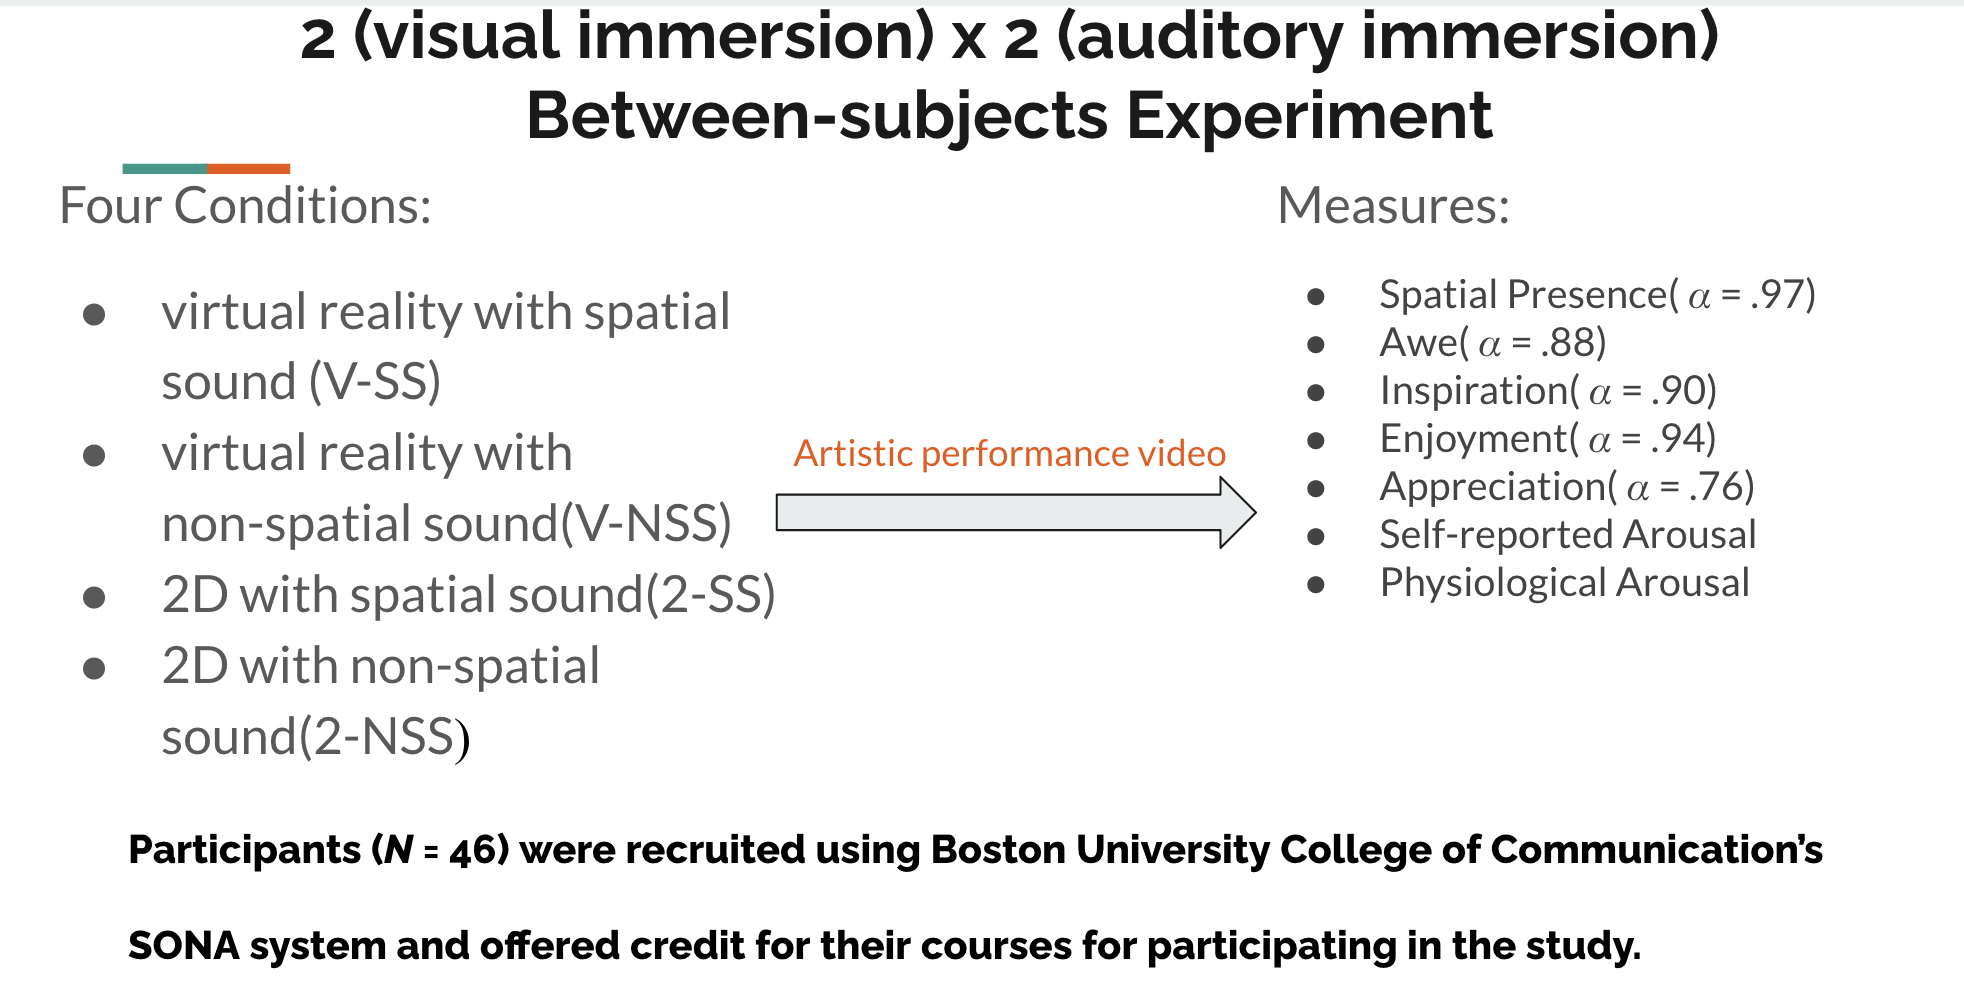
\includegraphics{3.png}
\caption{An overview of my previous study}
\end{figure}

To explore how audio/musical features might interact with the psychological effects of audio immersion in this process, the author downloaded data on about 30,000 Spotify songs from Kaggle, a popular online data science platform. This data was originally collected and updated from Spotify using the R package ``spotifyr'' \citep{kaggle30000spotify}. This dataset includes both production information about the songs (e.g., artists, song names, popularity, and release dates) as well as various musical features measured by Spotify (e.g., genre, danceability, valence).

Utilizing this data, the author aims to identify the key musical features that influence users' choices of study music on Spotify and determine whether these features contribute to a song's popularity. Additionally, the study will examine how these musical features are affected or enhanced by other musical characteristics. By exploring these research questions, the author intends to use insights from this analysis to guide the design of an experimental plan.

Here's an overview of this dataset with a brief explanation of each musical feature:

\begin{itemize}
\tightlist
\item
  \textbf{Danceability}: a track's suitability for dancing, based on tempo, rhythm stability, beat strength, and regularity. It ranges from 0.0 (least danceable) to 1.0 (most danceable).
\item
  \textbf{Energy}: a track's intensity and activity, on a scale of 0.0 to 1.0.
\item
  \textbf{Loudness}: overall loudness of a track in decibels (dB), averaged across the entire track, typically range from -60 to 0 dB.
\item
  \textbf{Speechiness}: detects spoken words presence in a track. Values closer to 1.0 indicate tracks composed mainly of speech. Values between 0.33 and 0.66 can include both music and speech, like rap music, while values below 0.33 are likely music or non-speech tracks.
\item
  \textbf{Acousticness}: a measure from 0.0 to 1.0 indicating whether a track is acoustic. A value of 1.0 represents high confidence in the track being acoustic.
\item
  \textbf{Instrumentalness}: predicts whether a track lacks vocals (ranging from 0.0 to 1.0). The closer the value is to 1.0, the more likely the track is purely instrumental.
\item
  \textbf{Liveness}: detects the presence of an audience in the recording, ranging from 0.0 to 1.0. Higher values indicate a higher probability of the track being performed live. A value above 0.8 suggests the track is likely live.
\item
  \textbf{Valence}: a measure from 0.0 to 1.0 that describes the musical positiveness conveyed by a track. High valence tracks sound positive (happy, cheerful), while low valence tracks sound negative (sad, angry).
\item
  \textbf{Tempo}: overall estimated tempo of a track in beats per minute (BPM), relating to the speed of the song.
\item
  \textbf{Duration}: length of the song, measured in milliseconds.
\end{itemize}

\begin{Shaded}
\begin{Highlighting}[]
\FunctionTok{summary}\NormalTok{(spotify)}
\end{Highlighting}
\end{Shaded}

\begin{verbatim}
##    track_id          track_name        track_artist       track_popularity
##  Length:32833       Length:32833       Length:32833       Min.   :  0.00  
##  Class :character   Class :character   Class :character   1st Qu.: 24.00  
##  Mode  :character   Mode  :character   Mode  :character   Median : 45.00  
##                                                           Mean   : 42.48  
##                                                           3rd Qu.: 62.00  
##                                                           Max.   :100.00  
##  track_album_id     track_album_name   track_album_release_date
##  Length:32833       Length:32833       Length:32833            
##  Class :character   Class :character   Class :character        
##  Mode  :character   Mode  :character   Mode  :character        
##                                                                
##                                                                
##                                                                
##  playlist_name      playlist_id        playlist_genre     playlist_subgenre 
##  Length:32833       Length:32833       Length:32833       Length:32833      
##  Class :character   Class :character   Class :character   Class :character  
##  Mode  :character   Mode  :character   Mode  :character   Mode  :character  
##                                                                             
##                                                                             
##                                                                             
##   danceability        energy              key            loudness      
##  Min.   :0.0000   Min.   :0.000175   Min.   : 0.000   Min.   :-46.448  
##  1st Qu.:0.5630   1st Qu.:0.581000   1st Qu.: 2.000   1st Qu.: -8.171  
##  Median :0.6720   Median :0.721000   Median : 6.000   Median : -6.166  
##  Mean   :0.6548   Mean   :0.698619   Mean   : 5.374   Mean   : -6.720  
##  3rd Qu.:0.7610   3rd Qu.:0.840000   3rd Qu.: 9.000   3rd Qu.: -4.645  
##  Max.   :0.9830   Max.   :1.000000   Max.   :11.000   Max.   :  1.275  
##       mode         speechiness      acousticness    instrumentalness   
##  Min.   :0.0000   Min.   :0.0000   Min.   :0.0000   Min.   :0.0000000  
##  1st Qu.:0.0000   1st Qu.:0.0410   1st Qu.:0.0151   1st Qu.:0.0000000  
##  Median :1.0000   Median :0.0625   Median :0.0804   Median :0.0000161  
##  Mean   :0.5657   Mean   :0.1071   Mean   :0.1753   Mean   :0.0847472  
##  3rd Qu.:1.0000   3rd Qu.:0.1320   3rd Qu.:0.2550   3rd Qu.:0.0048300  
##  Max.   :1.0000   Max.   :0.9180   Max.   :0.9940   Max.   :0.9940000  
##     liveness         valence           tempo         duration_ms    
##  Min.   :0.0000   Min.   :0.0000   Min.   :  0.00   Min.   :  4000  
##  1st Qu.:0.0927   1st Qu.:0.3310   1st Qu.: 99.96   1st Qu.:187819  
##  Median :0.1270   Median :0.5120   Median :121.98   Median :216000  
##  Mean   :0.1902   Mean   :0.5106   Mean   :120.88   Mean   :225800  
##  3rd Qu.:0.2480   3rd Qu.:0.6930   3rd Qu.:133.92   3rd Qu.:253585  
##  Max.   :0.9960   Max.   :0.9910   Max.   :239.44   Max.   :517810
\end{verbatim}

\hypertarget{electronic-dance-music-cognitive-flow}{%
\chapter{Electronic Dance Music \& Cognitive Flow}\label{electronic-dance-music-cognitive-flow}}

Although this report primarily seeks to identify the musical features that can induce cognitive flow, it is important to acknowledge that the composition of a song is a complex process. Users' listening experiences are significantly influenced by factors beyond musical features, such as the artists performing the songs and the overall quality of the song. To control for confounding variables that may affect users' cognitive flow state, and to maximize the mediating role of cognitive flow in leading to eudaimonia and self-transcendence, the genre of a song is utilized as a control variable in this study, especially considered how genres affect users' preferences and familiarity of music.

Here is a visualization showing the popularity/likability of different music genres by release year.

\begin{Shaded}
\begin{Highlighting}[]
\NormalTok{gg }\OtherTok{\textless{}{-}} \FunctionTok{ggplot}\NormalTok{(spotify\_data, }\FunctionTok{aes}\NormalTok{(}\AttributeTok{x =}\NormalTok{ release\_year, }\AttributeTok{y =}\NormalTok{ genre\_popularity, }\AttributeTok{group =}\NormalTok{ playlist\_genre, }\AttributeTok{color =}\NormalTok{ playlist\_genre)) }\SpecialCharTok{+}
  \FunctionTok{geom\_line}\NormalTok{() }\SpecialCharTok{+} \FunctionTok{geom\_point}\NormalTok{() }\SpecialCharTok{+}
  \FunctionTok{labs}\NormalTok{(}\AttributeTok{title =} \StringTok{"Genre Popularity Over Years"}\NormalTok{, }\AttributeTok{x =} \StringTok{"Year"}\NormalTok{, }\AttributeTok{y =} \StringTok{"Genre Popularity"}\NormalTok{) }\SpecialCharTok{+}
  \FunctionTok{theme\_minimal}\NormalTok{()}
\NormalTok{p }\OtherTok{\textless{}{-}} \FunctionTok{ggplotly}\NormalTok{(gg)}
\NormalTok{p}
\end{Highlighting}
\end{Shaded}

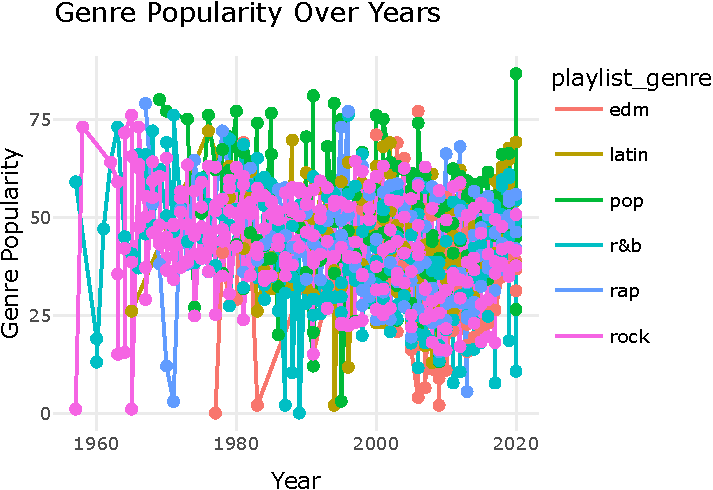
\includegraphics{_main_files/figure-latex/unnamed-chunk-4-1.pdf}

Based on this plot, it can be firstly understood that Spotify officially categorizes songs into six genres: electronic dance music, Latin music, pop music, rhythm \& blues, rap, and rock music.

\hypertarget{why-choose-edm-as-study-music}{%
\section{Why Choose EDM as Study Music}\label{why-choose-edm-as-study-music}}

\begin{figure}
\centering
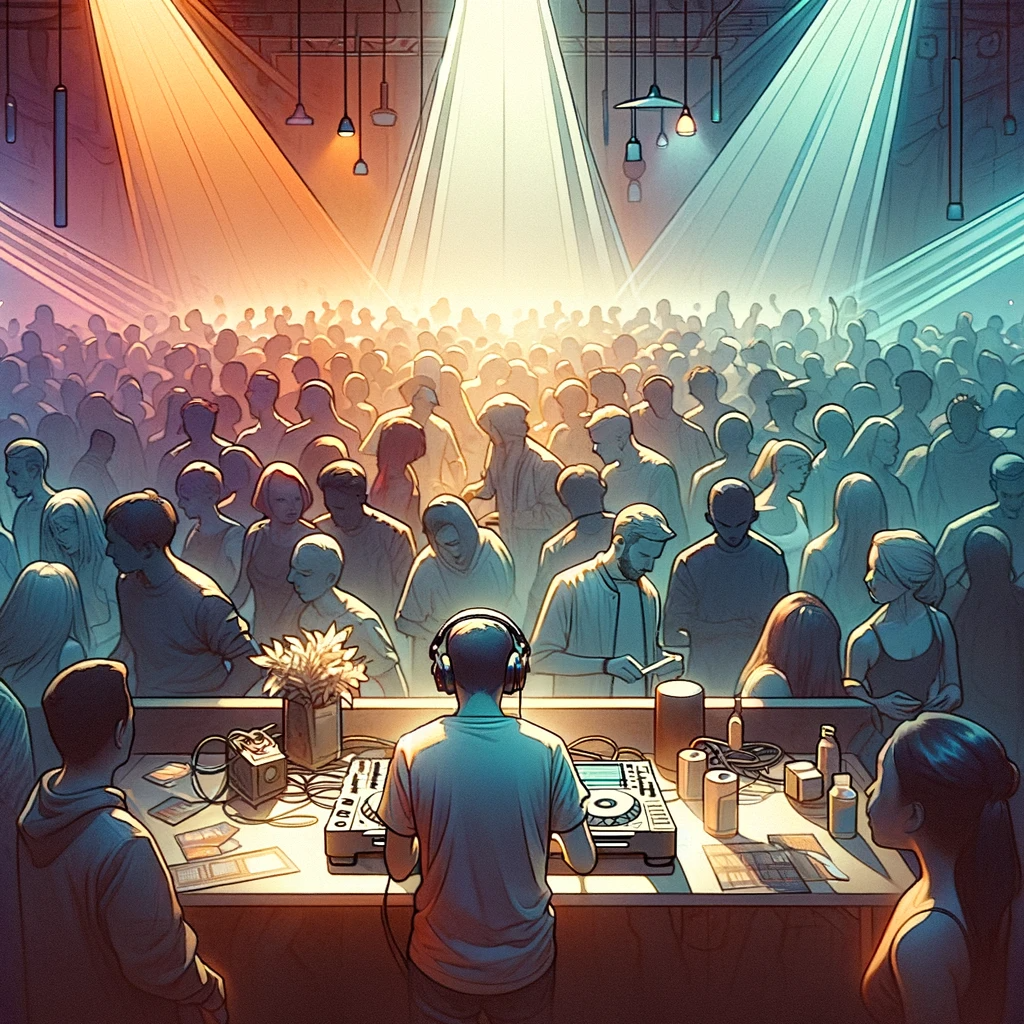
\includegraphics{4.png}
\caption{Electronic dance music}
\end{figure}

Both academic and industrial reports indicate that electronic dance music (EDM), including its subgenres like New Age/ambient EDM and trance/bass music, are frequently chosen as study music by users \citep[e.g.,][]{bosk2022electronic, dov2020positive, NationalUniversity2021}. These reports also highlight that ambient EDM music is often recommended as an optimal choice for study music because: 1) it typically has few or no lyrics, making it less distracting during study sessions; and 2) it is preferred by those who do not favor other types of instrumental music, such as classical music \citep{NationalUniversity2021}.

Furthermore, evidence from experimental studies suggests that there are optimal levels of tempo and energy in songs that influence their effectiveness in improving memory and learning \citep[e.g.,][]{musliu2017impact}.

Therefore, it can be assumed that:

\begin{itemize}
\tightlist
\item
  \textbf{H1}: Compared to other genres, EDM generally has a higher level of instrumentalness and a lower level of speechiness.
\end{itemize}

\begin{Shaded}
\begin{Highlighting}[]
\NormalTok{edm}\OtherTok{\textless{}{-}}\FunctionTok{subset}\NormalTok{(spotify, playlist\_genre}\SpecialCharTok{==}\StringTok{"edm"}\NormalTok{)}
\NormalTok{other\_genre }\OtherTok{\textless{}{-}} \FunctionTok{anti\_join}\NormalTok{(spotify, edm, }\AttributeTok{by =} \StringTok{"playlist\_genre"}\NormalTok{)}
\FunctionTok{t.test}\NormalTok{(edm}\SpecialCharTok{$}\NormalTok{instrumentalness,other\_genre}\SpecialCharTok{$}\NormalTok{instrumentalness,}\AttributeTok{paired=}\ConstantTok{FALSE}\NormalTok{,}\AttributeTok{alternative=}\StringTok{"greater"}\NormalTok{)}
\end{Highlighting}
\end{Shaded}

\begin{verbatim}
## 
##  Welch Two Sample t-test
## 
## data:  edm$instrumentalness and other_genre$instrumentalness
## t = 37.77, df = 6897.7, p-value < 2.2e-16
## alternative hypothesis: true difference in means is greater than 0
## 95 percent confidence interval:
##  0.156875      Inf
## sample estimates:
##  mean of x  mean of y 
## 0.21857790 0.05455906
\end{verbatim}

\begin{Shaded}
\begin{Highlighting}[]
\FunctionTok{t.test}\NormalTok{(edm}\SpecialCharTok{$}\NormalTok{speechiness,other\_genre}\SpecialCharTok{$}\NormalTok{speechiness,}\AttributeTok{paired=}\ConstantTok{FALSE}\NormalTok{,}\AttributeTok{alternative=}\StringTok{"less"}\NormalTok{)}
\end{Highlighting}
\end{Shaded}

\begin{verbatim}
## 
##  Welch Two Sample t-test
## 
## data:  edm$speechiness and other_genre$speechiness
## t = -22.258, df = 12955, p-value < 2.2e-16
## alternative hypothesis: true difference in means is less than 0
## 95 percent confidence interval:
##         -Inf -0.02312276
## sample estimates:
##  mean of x  mean of y 
## 0.08669548 0.11166350
\end{verbatim}

\begin{itemize}
\tightlist
\item
  \textbf{H2}: Compared to other genres, EDM generally exhibits different levels of a) tempo and b) energy.
\end{itemize}

\begin{Shaded}
\begin{Highlighting}[]
\FunctionTok{t.test}\NormalTok{(edm}\SpecialCharTok{$}\NormalTok{tempo,other\_genre}\SpecialCharTok{$}\NormalTok{tempo,}\AttributeTok{parired=}\ConstantTok{FALSE}\NormalTok{)}
\end{Highlighting}
\end{Shaded}

\begin{verbatim}
## 
##  Welch Two Sample t-test
## 
## data:  edm$tempo and other_genre$tempo
## t = 22.68, df = 17041, p-value < 2.2e-16
## alternative hypothesis: true difference in means is not equal to 0
## 95 percent confidence interval:
##  5.471608 6.506843
## sample estimates:
## mean of x mean of y 
##  125.7680  119.7788
\end{verbatim}

\begin{Shaded}
\begin{Highlighting}[]
\FunctionTok{t.test}\NormalTok{(edm}\SpecialCharTok{$}\NormalTok{energy,other\_genre}\SpecialCharTok{$}\NormalTok{energy,}\AttributeTok{parired=}\ConstantTok{FALSE}\NormalTok{)}
\end{Highlighting}
\end{Shaded}

\begin{verbatim}
## 
##  Welch Two Sample t-test
## 
## data:  edm$energy and other_genre$energy
## t = 60.415, df = 11144, p-value < 2.2e-16
## alternative hypothesis: true difference in means is not equal to 0
## 95 percent confidence interval:
##  0.1231538 0.1314133
## sample estimates:
## mean of x mean of y 
## 0.8024759 0.6751924
\end{verbatim}

Supported by two-sample t-tests, it could be concluded that given a 0.95 confidence level, EDM 1) compared to other genres, tends to have higher instrumentalness and lower speechiness, 2) exhibits distinct levels of tempo and energy compared to other genres. These results might support the idea that these audio features of EDM make it a favorable choice for study music

\hypertarget{edm-as-study-music-popularity}{%
\section{EDM as Study Music \& Popularity}\label{edm-as-study-music-popularity}}

Additionally, empirical evidence from experimental research indicates that musical activities with high levels of perceived pleasure and high engagement in movement can induce a cognitive flow state, particularly in a performance context \citep[e.g.,][]{loepthien2022flow}.

Given the observations show a significantly increasing preference for instrumental music, especially EDM, as background music during cognitive tasks on Spotify\citep[e.g.,][]{NationalUniversity2021, Spotify2021}, this trend could suggest that such preferences significantly drive the popularity of EDM songs.

If this ``bold hypothesis'' is considered valid, the following assumptions can be made:

\begin{itemize}
\item
  \textbf{H3}: EDM songs with higher levels of valence and danceability will have a higher popularity ranking.
\item
  \textbf{H4}: It can also be assumed, based on the ``popularity plot,'' that EDM songs released more recently will have a higher popularity ranking.
\end{itemize}

\begin{Shaded}
\begin{Highlighting}[]
\NormalTok{reg\_1}\OtherTok{\textless{}{-}}\FunctionTok{lm}\NormalTok{(track\_popularity}\SpecialCharTok{\textasciitilde{}}\NormalTok{release\_year}\SpecialCharTok{+}\NormalTok{danceability}\SpecialCharTok{+}\NormalTok{valence,edm)}
\FunctionTok{stargazer}\NormalTok{(reg\_1,}\AttributeTok{type=}\StringTok{"text"}\NormalTok{,}\AttributeTok{star.cutoffs=}\FunctionTok{c}\NormalTok{(.}\DecValTok{05}\NormalTok{,.}\DecValTok{01}\NormalTok{,.}\DecValTok{001}\NormalTok{))}
\end{Highlighting}
\end{Shaded}

\begin{verbatim}
## 
## =================================================
##                          Dependent variable:     
##                     -----------------------------
##                           track_popularity       
## -------------------------------------------------
## release_year                  1.869***           
##                                (0.087)           
##                                                  
## danceability                  -9.099***          
##                                (2.488)           
##                                                  
## valence                       17.389***          
##                                (1.365)           
##                                                  
## Constant                    -3,734.456***        
##                               (174.714)          
##                                                  
## -------------------------------------------------
## Observations                    6,043            
## R2                              0.088            
## Adjusted R2                     0.088            
## Residual Std. Error      22.117 (df = 6039)      
## F Statistic           194.241*** (df = 3; 6039)  
## =================================================
## Note:               *p<0.05; **p<0.01; ***p<0.001
\end{verbatim}

\begin{Shaded}
\begin{Highlighting}[]
\FunctionTok{plot}\NormalTok{(edm}\SpecialCharTok{$}\NormalTok{track\_popularity}\SpecialCharTok{\textasciitilde{}}\NormalTok{edm}\SpecialCharTok{$}\NormalTok{release\_year)}
\FunctionTok{abline}\NormalTok{(reg\_1)}
\end{Highlighting}
\end{Shaded}

\begin{verbatim}
## Warning in abline(reg_1): only using the first two of 4 regression coefficients
\end{verbatim}

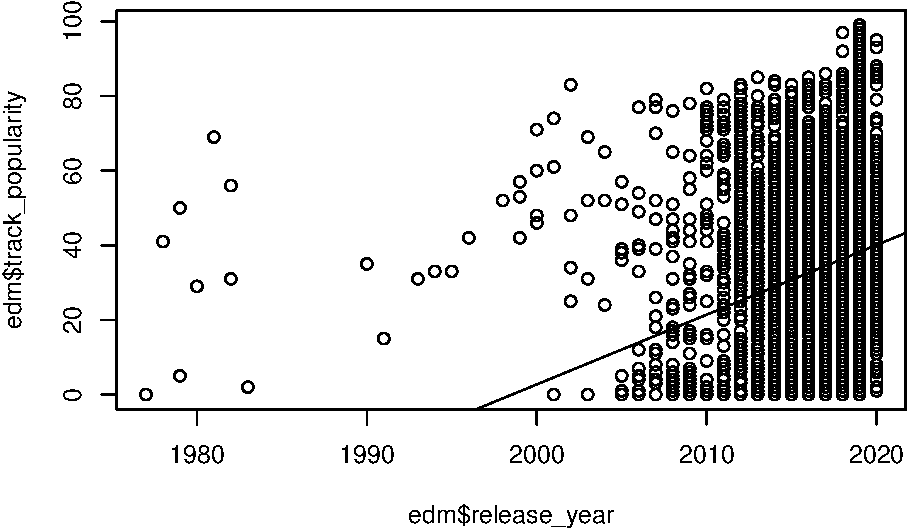
\includegraphics{_main_files/figure-latex/unnamed-chunk-8-1.pdf}

An interesting issue arises due to the sampling pattern of the ``spotifyr'' package. In the visualization example illustrating the relationship between track popularity and release year for EDM music, it is observed that:

\begin{itemize}
\item
  \textbf{Heteroscedasticity}: the variance of the residuals seems to increase with the increasing release year. This can be seen from the increasingly dispersed trend of the scatter plot, especially after the year 2000, where the dispersion of the residuals noticeably increases.
\item
  \textbf{Non-linear relationship}: the distribution of the data might suggests the possibility of a non-linear relationship.
\end{itemize}

Additionally, a Q-Q plot was utilized to examine whether the residual distribution approximate a normal distribution.

\begin{Shaded}
\begin{Highlighting}[]
\NormalTok{residuals\_1 }\OtherTok{\textless{}{-}}\NormalTok{ reg\_1}\SpecialCharTok{$}\NormalTok{residuals}
\FunctionTok{qqnorm}\NormalTok{(residuals\_1)}
\FunctionTok{qqline}\NormalTok{(residuals\_1, }\AttributeTok{col =} \StringTok{"red"}\NormalTok{,}\AttributeTok{lwd=}\DecValTok{2}\NormalTok{)}
\end{Highlighting}
\end{Shaded}

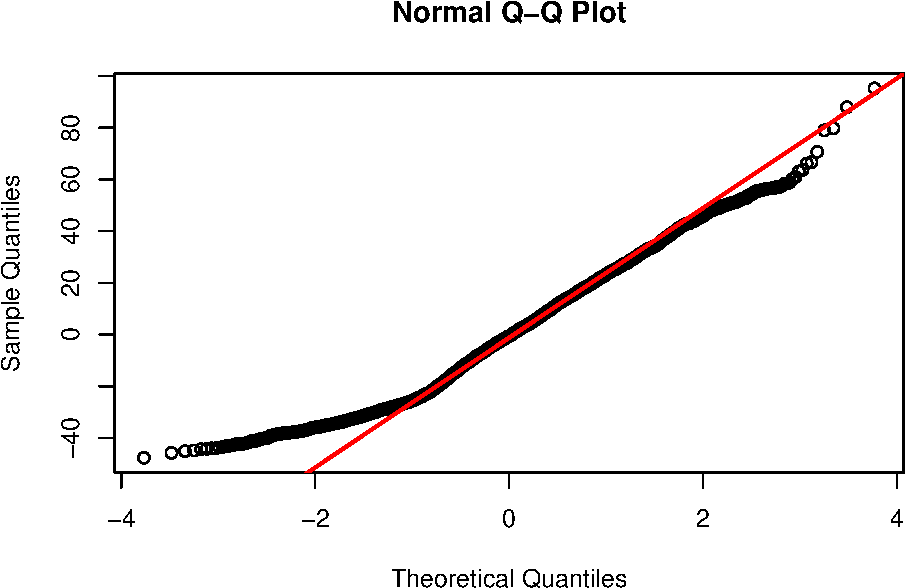
\includegraphics{_main_files/figure-latex/unnamed-chunk-9-1.pdf}

It can be seen from the points at the ends deviate from the reference line, especially at the right end of the plot, indicating potential skewness in the residual distribution at the extreme values of the data, suggesting that the tail weight of the residual distribution does not match that of a normal distribution.

It can be concluded that simple linear model might not be BLUE model here to examine the hypothesized relationship.

Additionally, a White'sRobust Standard Errors is utilized for correcting estimates of OLS regression coefficients of release year in the presence of heteroskedasticity.The adjustment resulted in a slightly different standard error for the release year coefficient.

\begin{Shaded}
\begin{Highlighting}[]
\NormalTok{robust\_1}\OtherTok{\textless{}{-}}\FunctionTok{vcovHC}\NormalTok{(reg\_1,}\StringTok{"HC1"}\NormalTok{)}
\NormalTok{result\_1}\OtherTok{\textless{}{-}}\FunctionTok{coeftest}\NormalTok{(reg\_1,robust\_1)}
\NormalTok{result\_1[}\StringTok{"release\_year"}\NormalTok{,]}
\end{Highlighting}
\end{Shaded}

\begin{verbatim}
##     Estimate   Std. Error      t value     Pr(>|t|) 
## 1.868585e+00 1.417803e-01 1.317944e+01 3.981126e-39
\end{verbatim}

\begin{Shaded}
\begin{Highlighting}[]
\FunctionTok{summary}\NormalTok{(reg\_1)}
\end{Highlighting}
\end{Shaded}

\begin{verbatim}
## 
## Call:
## lm(formula = track_popularity ~ release_year + danceability + 
##     valence, data = edm)
## 
## Residuals:
##    Min     1Q Median     3Q    Max 
## -47.65 -18.15  -0.60  15.68  95.25 
## 
## Coefficients:
##                Estimate Std. Error t value Pr(>|t|)    
## (Intercept)  -3.734e+03  1.747e+02 -21.375  < 2e-16 ***
## release_year  1.869e+00  8.661e-02  21.574  < 2e-16 ***
## danceability -9.099e+00  2.488e+00  -3.657 0.000257 ***
## valence       1.739e+01  1.365e+00  12.741  < 2e-16 ***
## ---
## Signif. codes:  0 '***' 0.001 '**' 0.01 '*' 0.05 '.' 0.1 ' ' 1
## 
## Residual standard error: 22.12 on 6039 degrees of freedom
## Multiple R-squared:  0.088,  Adjusted R-squared:  0.08755 
## F-statistic: 194.2 on 3 and 6039 DF,  p-value: < 2.2e-16
\end{verbatim}

\hypertarget{conclusion-from-ols}{%
\subsection{Conclusion From OLS}\label{conclusion-from-ols}}

Although the results from OLS suggest that simple linear model might not be the best fit for the given data, it can still be concluded from the OLS regressions that:

-\textbf{1. Release Year}: holding other variables constant, for each additional release year, the popularity scores of EDM songs increases by approximately 1.869 points, suggesting newer EDM songs tend to be more popular, supporting hypothesis 4.

-\textbf{2. Danceability}: contrary to what might be expected, a significant but negative relationship between danceability feature and track popularity score. For each additional 0.1 increase in danceability score, the track's popularity would decrease by approximately 0.9099 points.

-\textbf{3. Valence}: a significant and strongly positive relationship exists between valence and track popularity score, predicted by the model. Holding others constant, for each additioanl 0.1 increase in valence score, the track's popularity scores would increase by approximately 1.7389 points.

-\textbf{4. R-squared}: approximately only 8.8\% of the variability in track popularity can be explained when utilizing a simple linear model.

-\textbf{5. F Statistic}: with a 194.24 f-statistic score, indicating that the model as a whole is statistically significant.

Overall, the OLS regression supports Hypothesis 4 (H4) and partially supports Hypothesis 3 (H3). Contrary to the original hypothesis regarding the relationship between danceability and popularity, this might be due to two reasons: 1) Danceability might be inversely correlated with other musical features that affect popularity. 2) Users in a studying context might prefer less danceable tracks for background listening. Additionally, issues with model fit, as indicated by the residual analysis and regression diagnostics, suggest that further investigation with more complex models or additional variables might be necessary for a more comprehensive understanding of what drives the popularity of EDM songs.

\hypertarget{further-exploration-on-key-musical-features-danceability}{%
\chapter{Further Exploration on Key Musical Features: danceability}\label{further-exploration-on-key-musical-features-danceability}}

\hypertarget{interpretation-testing}{%
\section{Interpretation Testing}\label{interpretation-testing}}

To gain an in-depth understanding of the results for Hypothesis 3 (H3), OLS regression analysis was utilized to test the relationship between danceability and track popularity/valence. This was done in light of various existing evidence that supports the notion that people prefer tracks they can dance or move to, in relation to their reasons for listening. \citep[e.g.,][]{duman2022music, loepthien2022flow}

Additionally, it is interesting to explore the potential relationship between valence and danceability of an EDM song, especially considering evidence indicating that dance music typically has a higher level of valence.

\begin{itemize}
\tightlist
\item
  \textbf{H5}: A higher level of danceability in an EDM song will predict a higher level of perceived valence for the song.
\end{itemize}

\begin{Shaded}
\begin{Highlighting}[]
\NormalTok{reg\_2}\OtherTok{\textless{}{-}}\FunctionTok{lm}\NormalTok{(track\_popularity}\SpecialCharTok{\textasciitilde{}}\NormalTok{danceability,edm)}
\NormalTok{reg\_3}\OtherTok{\textless{}{-}}\FunctionTok{lm}\NormalTok{(valence}\SpecialCharTok{\textasciitilde{}}\NormalTok{danceability,edm)}
\FunctionTok{stargazer}\NormalTok{(reg\_2,reg\_3,}\AttributeTok{type=}\StringTok{"text"}\NormalTok{,}\AttributeTok{star.cutoffs=}\FunctionTok{c}\NormalTok{(.}\DecValTok{05}\NormalTok{,.}\DecValTok{01}\NormalTok{,.}\DecValTok{001}\NormalTok{))}
\end{Highlighting}
\end{Shaded}

\begin{verbatim}
## 
## ==============================================================
##                                      Dependent variable:      
##                                 ------------------------------
##                                 track_popularity    valence   
##                                        (1)            (2)     
## --------------------------------------------------------------
## danceability                          1.403         0.693***  
##                                      (2.411)        (0.022)   
##                                                               
## Constant                            33.914***      -0.053***  
##                                      (1.607)        (0.015)   
##                                                               
## --------------------------------------------------------------
## Observations                          6,043          6,043    
## R2                                   0.0001          0.143    
## Adjusted R2                          -0.0001         0.143    
## Residual Std. Error (df = 6041)      23.156          0.209    
## F Statistic (df = 1; 6041)            0.339       1,010.744***
## ==============================================================
## Note:                            *p<0.05; **p<0.01; ***p<0.001
\end{verbatim}

From the results, it can be concluded that when holding other variables constant, the danceability of EDM songs and corresponding track popularity do not exhibit a clear correlational relationship. Additionally, in line with expectations, valence and danceability show a clear positive correlation, as a higher level of danceability in an EDM song leads to higher perceived valence, supporting H5.

If the hypothesis that users increasingly choose EDM as study music significantly drives the popularity of this genre holds valid, the combination of these results suggests that danceability might be inversely correlated with other musical features that affect popularity.

\hypertarget{interaction-effects-of-danceability-and-loudness-on-popularity}{%
\section{Interaction Effects of Danceability and Loudness on Popularity}\label{interaction-effects-of-danceability-and-loudness-on-popularity}}

evidence from previous studies on background music' cognitive effect suggests that noise (i.e., extreme loudness) of background music are considered significantly affect workers' attention \citep[e.g.,][]{shih2012background}

As fewer studies have suggested a relationship between the danceability of a song and its loudness, the following research questions are proposed:

\begin{itemize}
\item
  \textbf{RQ1}: What is the relationship between the danceability and the loudness of an EDM song?
\item
  \textbf{RQ2}: Does the relationship between the danceability of EDM songs and their corresponding track popularity depend on the loudness level of those songs?
\end{itemize}

\begin{Shaded}
\begin{Highlighting}[]
\NormalTok{reg\_4}\OtherTok{\textless{}{-}}\FunctionTok{lm}\NormalTok{(danceability}\SpecialCharTok{\textasciitilde{}}\NormalTok{loudness,edm)}
\NormalTok{reg\_5}\OtherTok{\textless{}{-}}\FunctionTok{lm}\NormalTok{(track\_popularity}\SpecialCharTok{\textasciitilde{}}\NormalTok{loudness}\SpecialCharTok{+}\NormalTok{danceability}\SpecialCharTok{+}\NormalTok{loudness}\SpecialCharTok{*}\NormalTok{danceability,edm)}
\FunctionTok{stargazer}\NormalTok{(reg\_4,reg\_5,}\AttributeTok{type=}\StringTok{"text"}\NormalTok{,}\AttributeTok{star.cutoffs=}\FunctionTok{c}\NormalTok{(.}\DecValTok{05}\NormalTok{,.}\DecValTok{01}\NormalTok{,.}\DecValTok{001}\NormalTok{))}
\end{Highlighting}
\end{Shaded}

\begin{verbatim}
## 
## ======================================================================
##                                     Dependent variable:               
##                       ------------------------------------------------
##                             danceability           track_popularity   
##                                  (1)                     (2)          
## ----------------------------------------------------------------------
## loudness                      -0.010***                -2.186**       
##                                (0.001)                 (0.705)        
##                                                                       
## danceability                                          21.559***       
##                                                        (6.145)        
##                                                                       
## loudness:danceability                                  3.524***       
##                                                        (1.022)        
##                                                                       
## Constant                      0.602***                21.567***       
##                                (0.004)                 (4.110)        
##                                                                       
## ----------------------------------------------------------------------
## Observations                    6,043                   6,043         
## R2                              0.035                   0.002         
## Adjusted R2                     0.035                   0.002         
## Residual Std. Error       0.121 (df = 6041)       23.132 (df = 6039)  
## F Statistic           217.638*** (df = 1; 6041) 4.917** (df = 3; 6039)
## ======================================================================
## Note:                                    *p<0.05; **p<0.01; ***p<0.001
\end{verbatim}

From the analysis, it can be concluded that:

For RQ1, the loudness of an EDM song has only a slight correlational relationship with its danceability, with an estimated coefficient of -0.010.

For RQ2, while the results indicate that the effect of danceability on an EDM song's popularity is somewhat contingent on the song's loudness level, the very low R-squared value (0.002437) suggests that the variance in the popularity of an EDM song is hardly captured when considering only danceability and loudness in a simple linear regression model. Additionally, given a baseline constant coefficient of 21.567, it might be plausible that due to the inherently high danceability nature of the genre, increasing the danceability might not significantly affect how users choose different songs of such genres as study music.

\hypertarget{conclusion}{%
\chapter{Conclusion}\label{conclusion}}

This report delved into the key musical features that influence users' preferences for EDM as study music on Spotify. Features such as instrumentalness, optimal levels of tempo and energy, and the valence of a song appear to play pivotal roles in determining users' preferences for an EDM track. Notably, danceability, often considered highly associated with a song's suitability as background music in cognitive tasks, exhibited a complex correlation with a track's popularity in this context. These insights offer valuable guidance for the design of conditions and exposure in an upcoming experimental study focusing on audio features, cognitive performance, and eudaimonia.

A significant limitation of this study is the exclusive use of a simple linear regression model to test hypothesized relationships. The results suggest that more complex mathematical models would be better suited to address the given hypotheses and research questions.

Another limitation is the reliance on the assumption that an increasing preference for EDM as background music during cognitive tasks significantly drives the popularity of EDM songs. However, given the limitations of this data, this fundamental hypothesis cannot be tested.

Looking forward, this research can inform the development of more tailored and effective study music genres and audio features to enhance cognitive performance.

  \bibliography{book.bib,packages.bib}

\end{document}
